\newpage
\section{Results}
\subsection{Mean transverse momentum}

Figure~\ref{fig:mean_pt_vs_mult} shows the mean transverse momentum $\mpt$ as a function of mean 
charged-particle multiplicity density $\langle$d$N_{\mathrm{ch}}$/d$\eta_{\mathrm{lab}}\rangle$ at midrapidity.
The results for \xis are compared with those for other hyperons observed in p--Pb collisions at \snn = 5.02~TeV~\cite{cite:lambda_pPb, cite:Xi_pPb}.

\begin{figure}[htbp]
\begin{center}
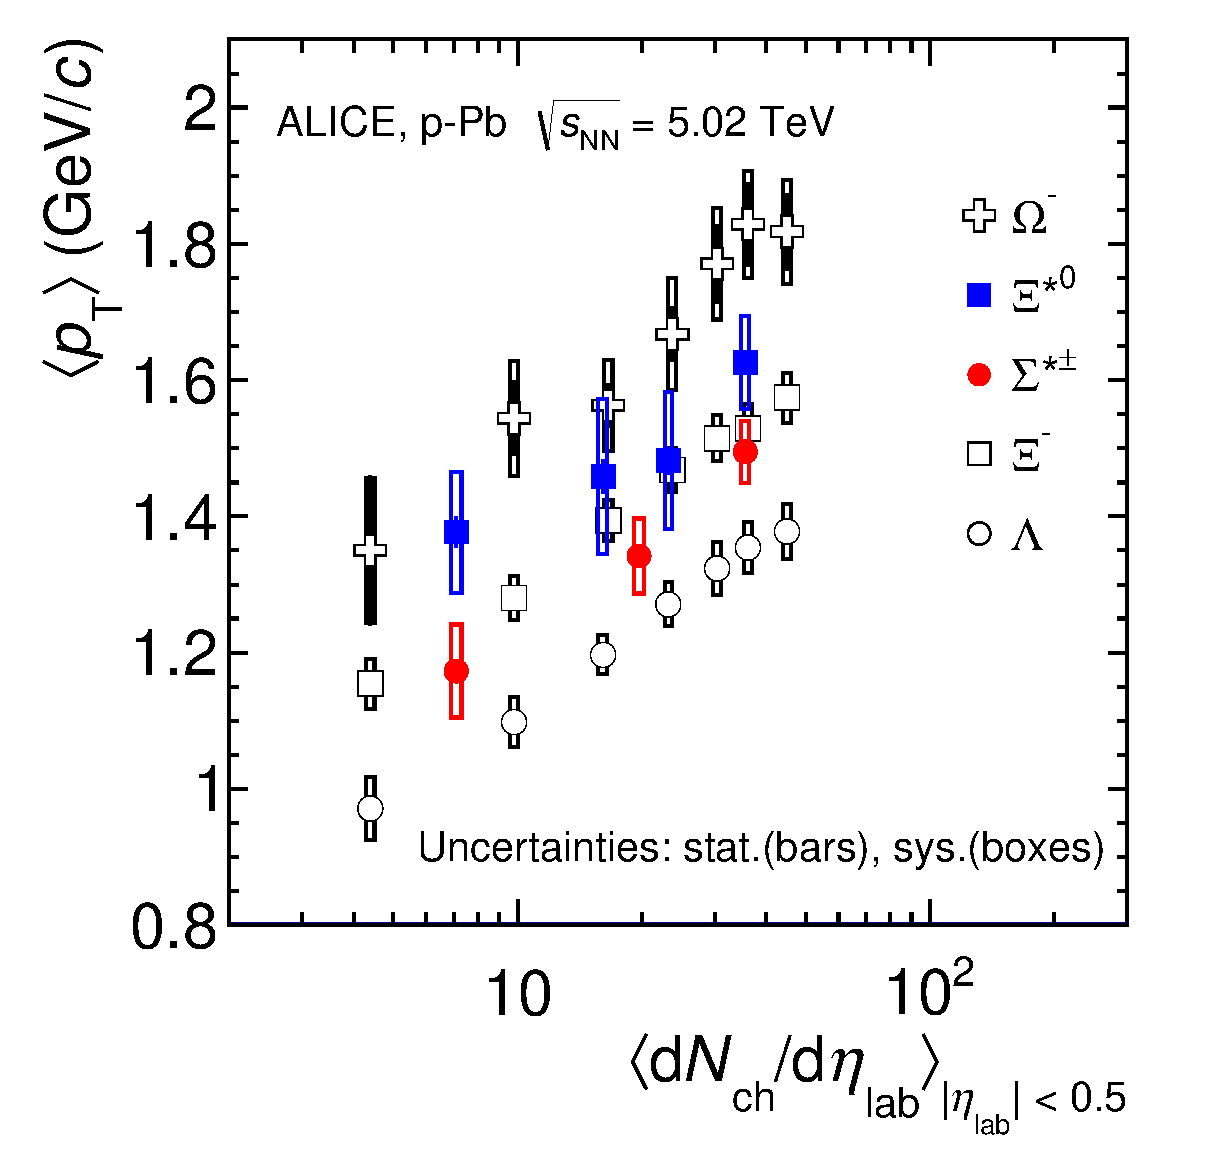
\includegraphics[width=10.cm]{./Version1/FigChapter6/mpt/mpt_mult.eps}
\caption{Mean transverse momenta $\mpt$ of $\Lambda$, $\Xi^{-}$, $\Sigma^{*\pm}$, $\Xi^{*0}$ 
  and $\Omega^{-}$ in p--Pb collisions at \snn = 5.02 TeV as a 
  function of mean charged-particle multiplicity density 
  $\langle$d$N_{\mathrm{ch}}$/d$\eta_{\mathrm{lab}}\rangle$, measured in the pseudorapidity range 
  $\mid\eta_{\mathrm{lab}}\mid <$~0.5. The results for $\Lambda$, $\Xi^{-}$ and $\Omega^{-}$ are taken 
  from~\cite{cite:lambda_pPb, cite:KphipPb, cite:Xi_pPb}. Statistical and systematic uncertainties are represented as bars 
  and boxes, respectively. The $\Omega^-$ and $\Xi^-$ points in the 3rd and 4th lowest multiplicity bins are slightly 
  displaced along the abscissa to avoid superposition with the \xis points.}
  \label{fig:mean_pt_vs_mult}
  \end{center}
\end{figure}


Increasing trends from low to high multiplicities are observed for all hyperons. The mean transverse momenta increase by 20\% as the mean charged-particle multiplicity increases from 7.1 to 35.6. This result is similar to the one obtained for the other hyperons. Furthermore, a similar increase has been observed also for K$^{\pm}$, K$_{\rm{S}}^{0}$, K$^{*}(892)^0$ and $\phi$~\cite{cite:KphipPb}, whereas protons are subject to a larger ($\sim$ 33\%) increase in the given multiplicity range, as discussed also in Ref.~\cite{cite:lambda_pPb}. 


\begin{figure}[htbp]
\begin{center}
\includegraphics[width=10.cm]{./Version1/FigChapter6/mpt/mpt_mass.eps}
\caption{Mass dependence of the mean transverse momenta of identified particles for the $0-20$\% V0A multiplicity class and with $-0.5<y_{\mathrm{CMS}}<0$ in p--Pb~collisions at \snn = 5.02 TeV~\cite{cite:lambda_pPb, cite:Xi_pPb}, and 
  in minimum-bias pp collisions at $\sqrt{s}$~=~7~TeV~\cite{cite:Xi_pp} with $|y_{\mathrm{CMS}}|<0.5$. Additionally, $D^0$ and $J$/$\psi$ results are plotted. The $D^0$ and $J$/$\psi$ were measured in different rapidity ranges: $|y_{\mathrm{CMS}}|<0.5$~\cite{cite:D0} 
  ($|y_{\mathrm{CMS}}|<0.9$~\cite{cite:Jpsi_pp}) for $D^0$ ($J$/$\psi$) in pp and $-0.96 < y_{\mathrm{CMS}}< 0.04$~\cite{cite:D0} ($-1.37<y_{\mathrm{CMS}}<0.43$~\cite{cite:Jpsi_pPb}) 
  for $D^0$ ($J$/$\psi$) in p--Pb. Note also that the results for $D^0$ and $J$/$\psi$ in p-Pb collisions are for the 0-100\% multiplicity class.}
  \label{fig:mean_pt_vs_mass}
 \end{center}
\end{figure}

In all multiplicity classes, the $\mpt$ follows an approximate mass ordering: 
$\mpt_{\Lambda}<\mpt_{\Xi^-}$~$\simeq$~$\mpt_{\Sigma^{*\pm}}<\mpt_{\Xi^{*0}}<\mpt_{\Omega^{-}}$.
The $\mpt$ of $\Sigma^{*\pm}$ looks systematically lower than the $\mpt$ of $\Xi^{-}$, despite the larger mass of 
$\Sigma^{*\pm}$. The uncertainties, however, are too large to draw any conclusion on 
possible hints of violation of the mass hierarchy. This hierarchy of mass-ordering, also including $D^0$ and 
$J$/$\psi$ in the comparison, is displayed in Figure \ref{fig:mean_pt_vs_mass}. Note, however, that the $D^0$ and $J$/$\psi$ were 
measured in different rapidity ranges: $|y_{\mathrm{CMS}}|<0.5$~\cite{cite:D0} ($|y_{\mathrm{CMS}}|<0.9$~\cite{cite:Jpsi_pp}) for $D^0$ ($J$/$\psi$) in pp and $-0.96 < y_{\mathrm{CMS}}< 0.04$~\cite{cite:D0} ($-1.37<y_{\mathrm{CMS}}<0.43$~\cite{cite:Jpsi_pPb}) for $D^0$ ($J$/$\psi$) in p--Pb, and the results for $D^0$ and $J$/$\psi$ in p-Pb collisions are for the 0-100\% multiplicity class. This mass dependence is observed in both p--Pb and pp collisions. 
It was observed also by the STAR collaboration~\cite{cite:STAR-hadronic_resonances-dAu} in MB pp, MB d--Au and central Au--Au collisions. 

Furthermore, for the light-flavour hadrons, the mean transverse momenta in p--Pb collisions are observed to be consistently higher than those in pp collisions at 7 TeV. The situation for the charm hadrons is different, where $\mpt$ appears compatible between both colliding systems. The discrepancy is likely due to different production mechanisms for heavy and light flavours and to a harder fragmentation of charm quarks. Specifically, the fact that $\mpt$ remains similar in pp and in p--Pb is consistent with an $R_{\mathrm{pPb}}$ ratio compatible with unity at all \pt \cite{cite:D0} for $D^0$, and/or 
with the effects of shadowing in p--Pb which reduces the production at low \pt and thus increasing the overall $\mpt$ for $J$/$\psi$~\cite{cite:Jpsi_pPb}; the small \pt hardening expected in pp when going from 5.02 to 7TeV is apparently not enough to counter-balance the situation.

Because of small decrease of the $\mpt$ for proton and $\Lambda$ relative to those for K$^{*0}$ and $\phi$, two different trends for mesons and baryons have been suggested~\cite{cite:mass_scaling}. Even including $D^0$ and $J$/$\psi$, as shown in Figure ~\ref{fig:mean_pt_vs_mass}, a different trend for 
mesons and baryons cannot be convincingly established.



\subsection{Particle yield ratios}
\begin{figure}[htbp]
\begin{center}
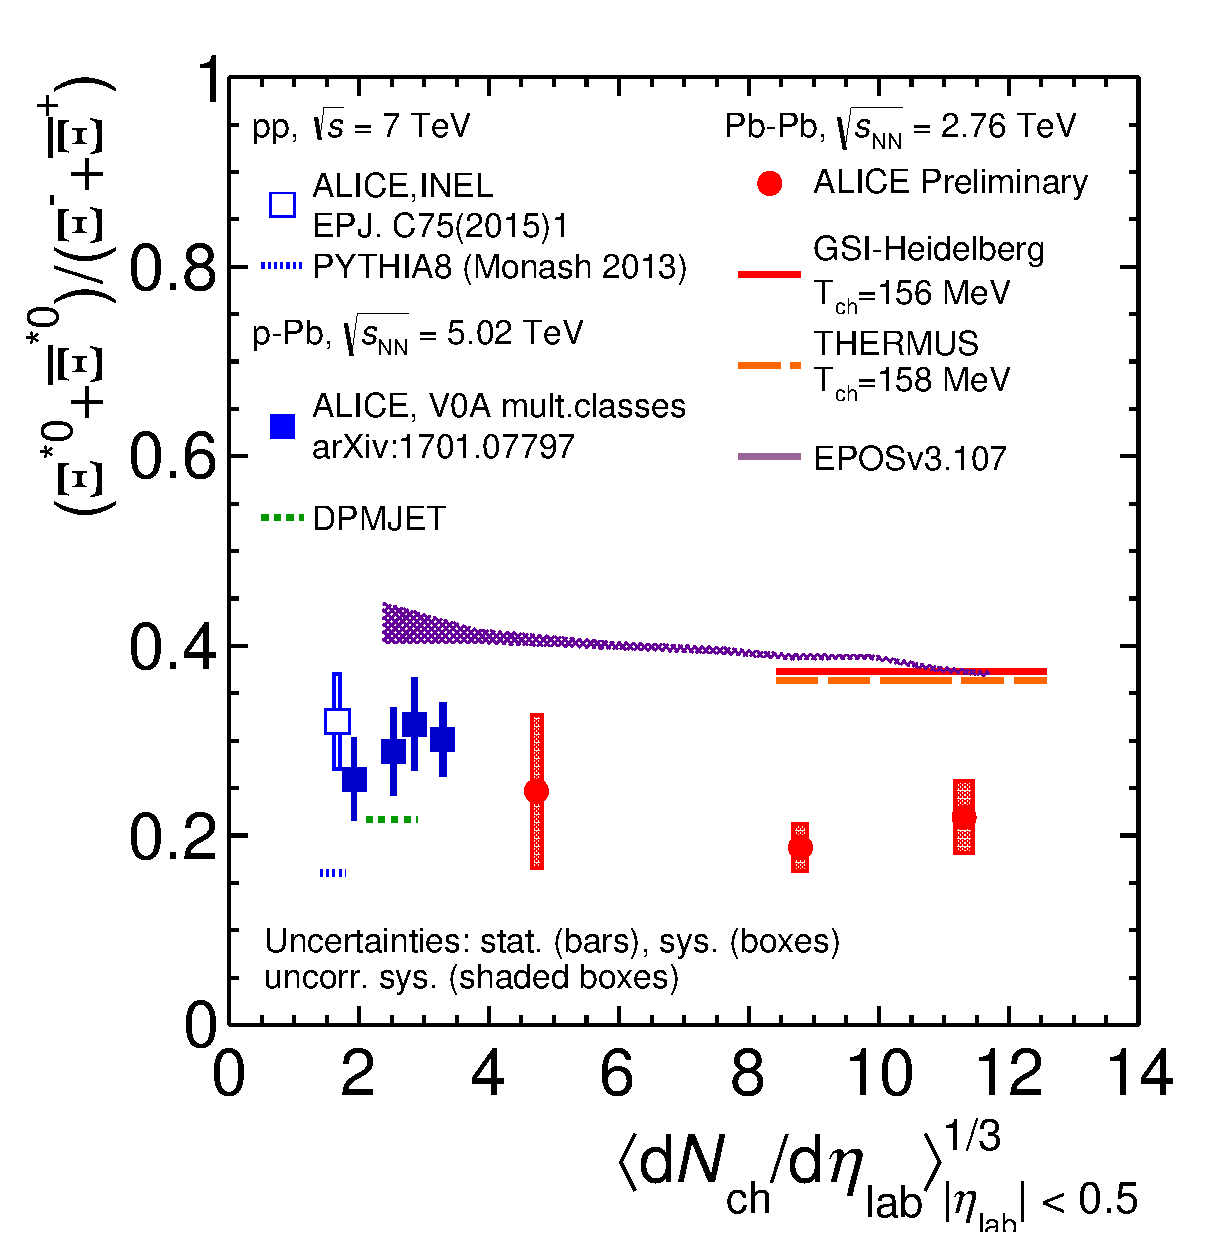
\includegraphics[width=12.cm]{./Version1/FigChapter6/Ratio/Ratio_XiStarToXi}
\caption{Integrated.}
\label{fig:xitoxi}
\end{center}
\end{figure}

\begin{figure}[htbp]
\begin{center}
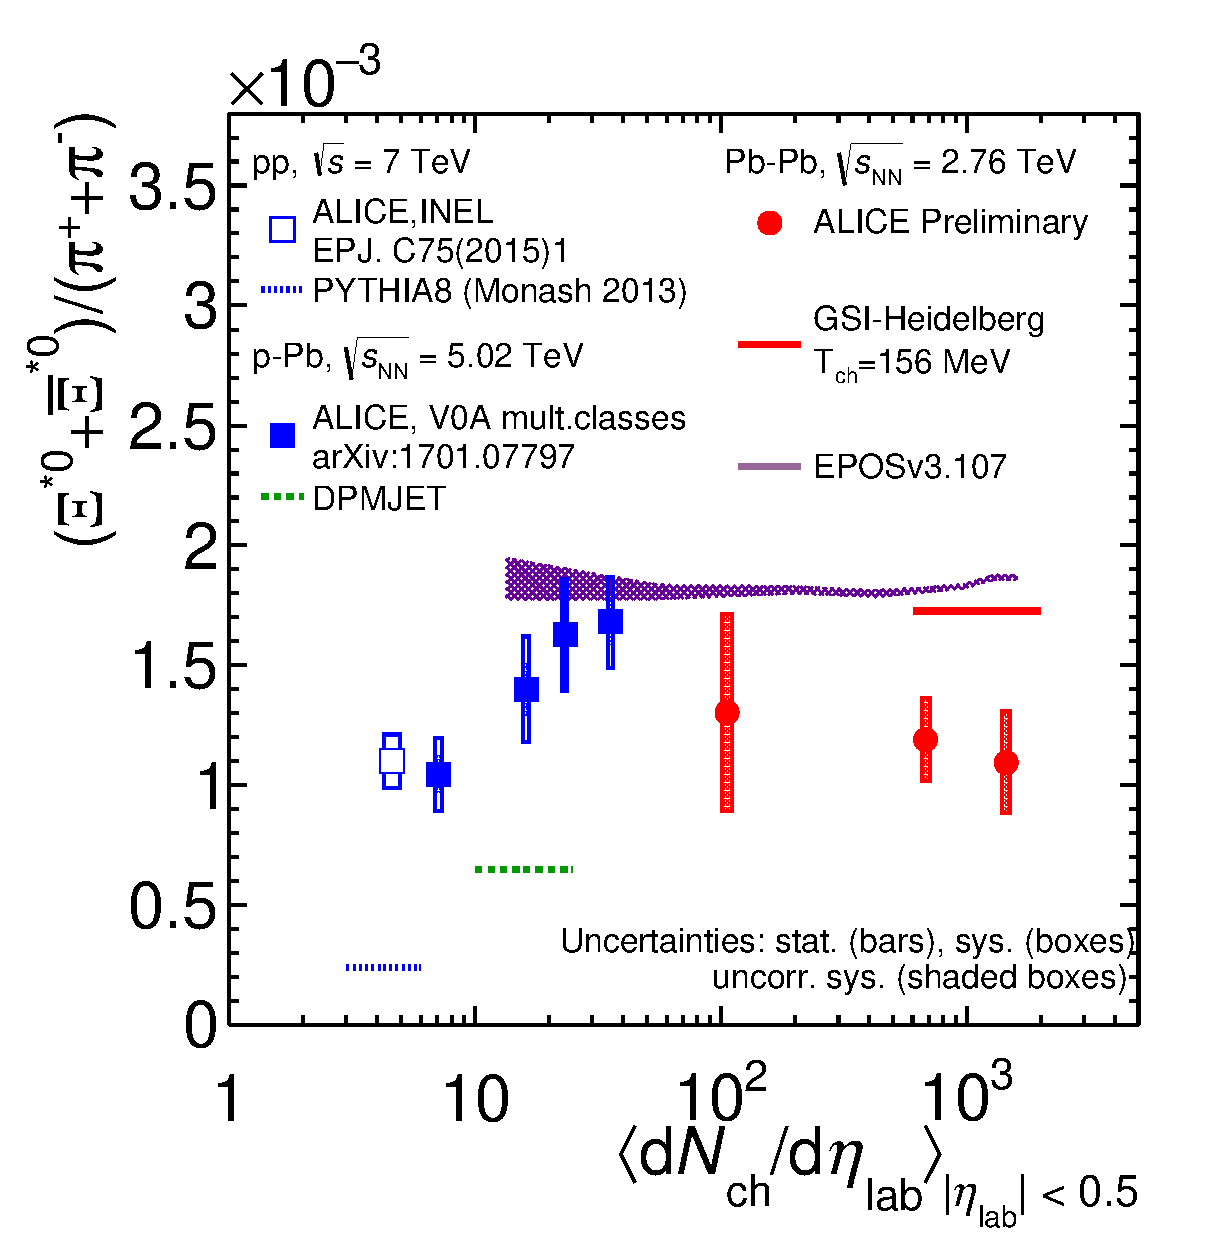
\includegraphics[width=12.cm]{./Version1/FigChapter6/Ratio/Ratio_XiStarToPion}
\caption{Integrated.}
\label{fig:xitopi}
\end{center}
\end{figure}

\subsubsection{Comparison with other resonances}
\subsubsection{Comparison with models}